\documentclass{standalone}

\begin{document}

\subsection[miRNA and RPPA data]{miRNA and RPPA dataset}\label{synapse:miRNA}

The same analysis pipeline presented in the paper about gene expression data from the Synapse dataset is applied in this Section also to the miRNA and RPPA datasets, with the results presented in Fig.~\ref{fig:other_results}.

\begin{figure}[htbp]
\centering
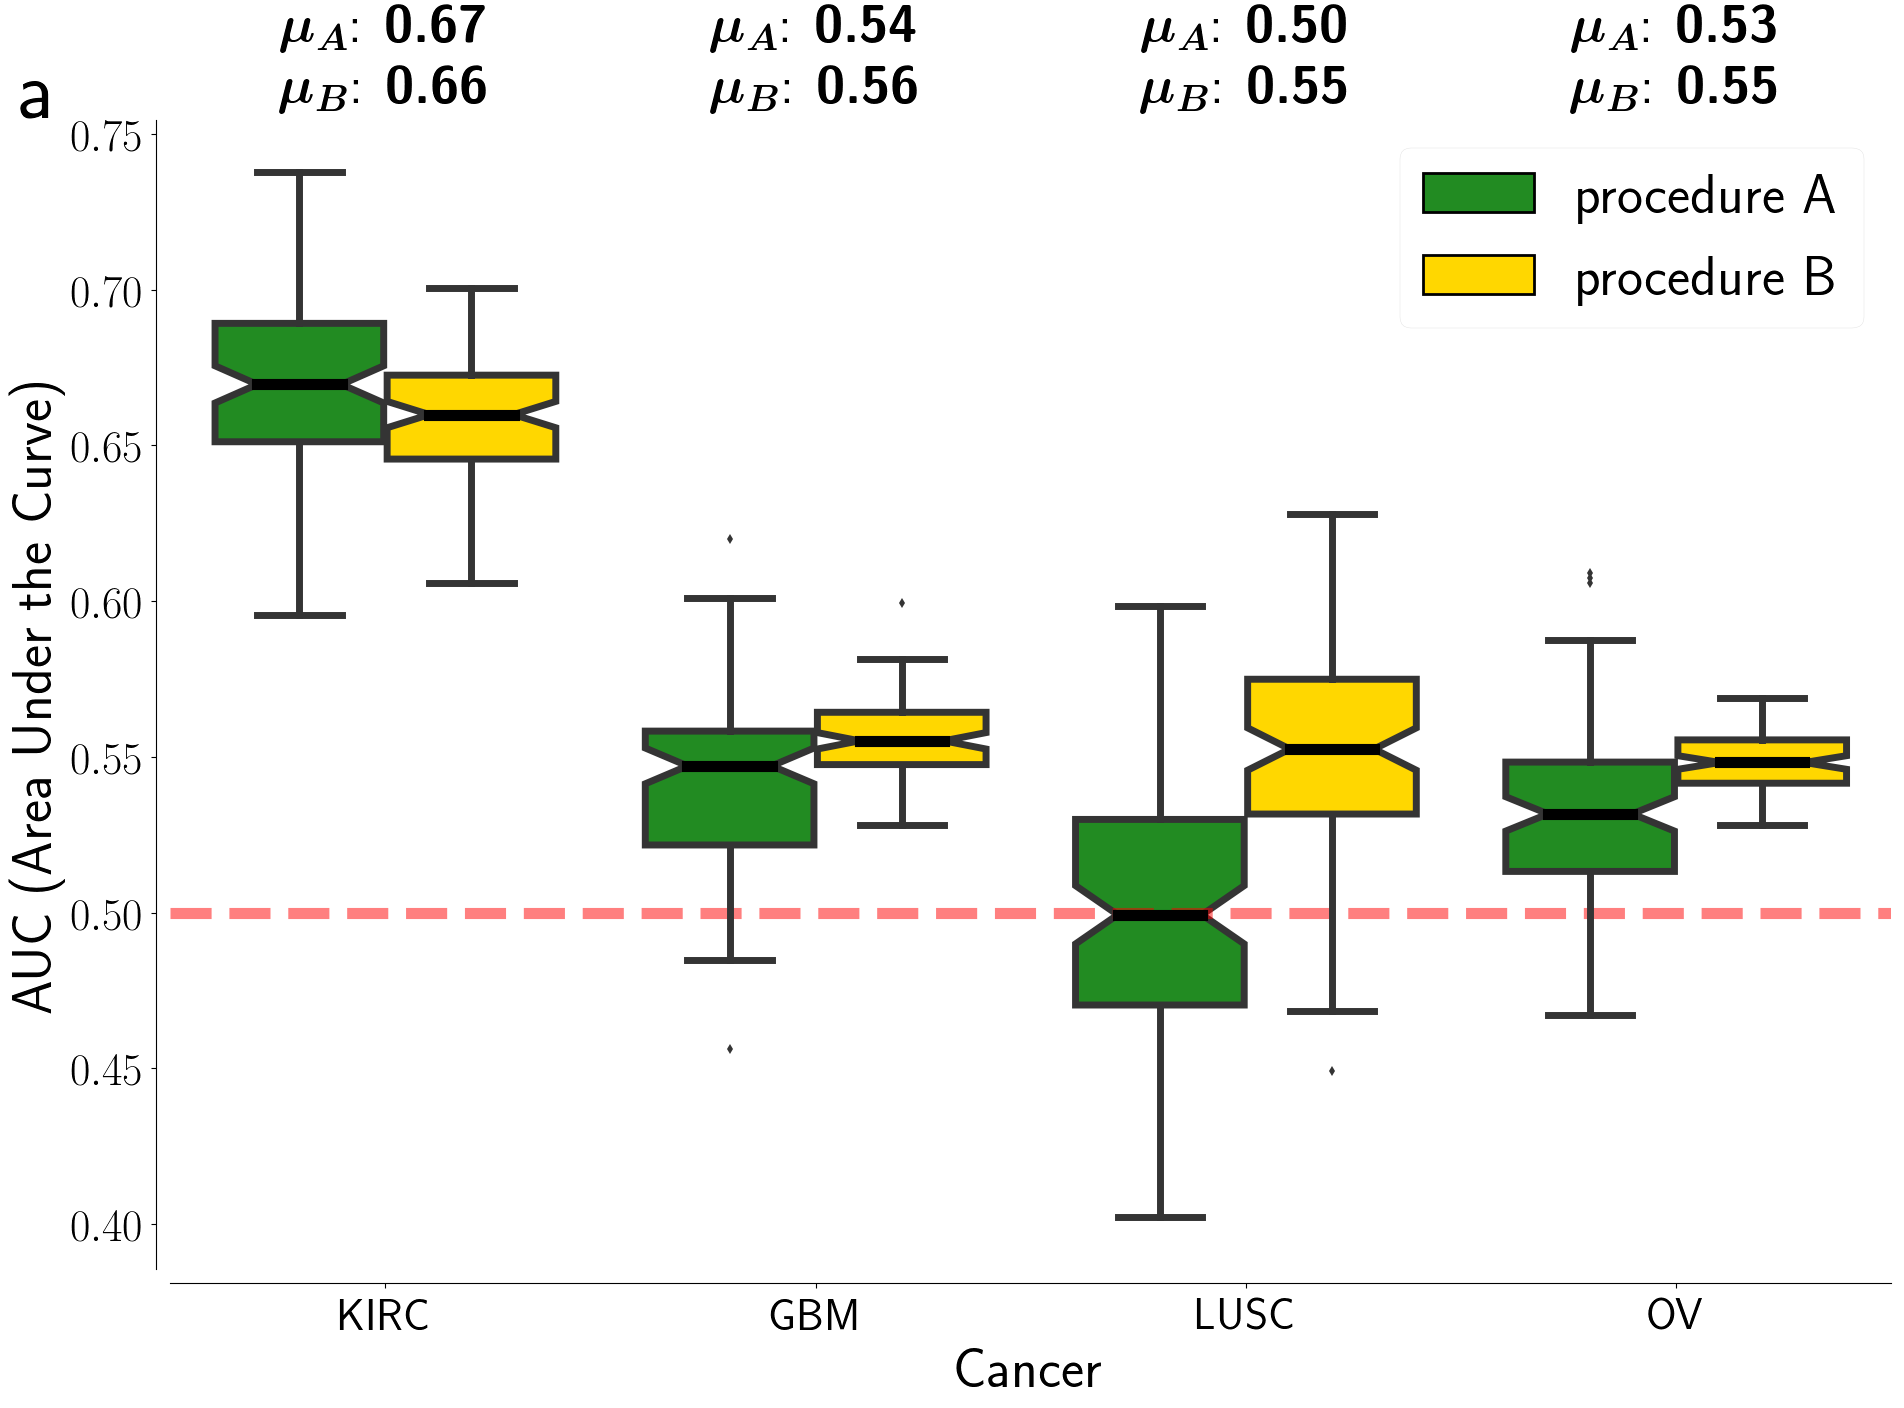
\includegraphics[width=0.4\textwidth]{miRNA_boxplot.png}
\qquad
\def\svgwidth{0.45\textwidth}
\input{./img/miRNA_tables.pdf_tex}
\newline
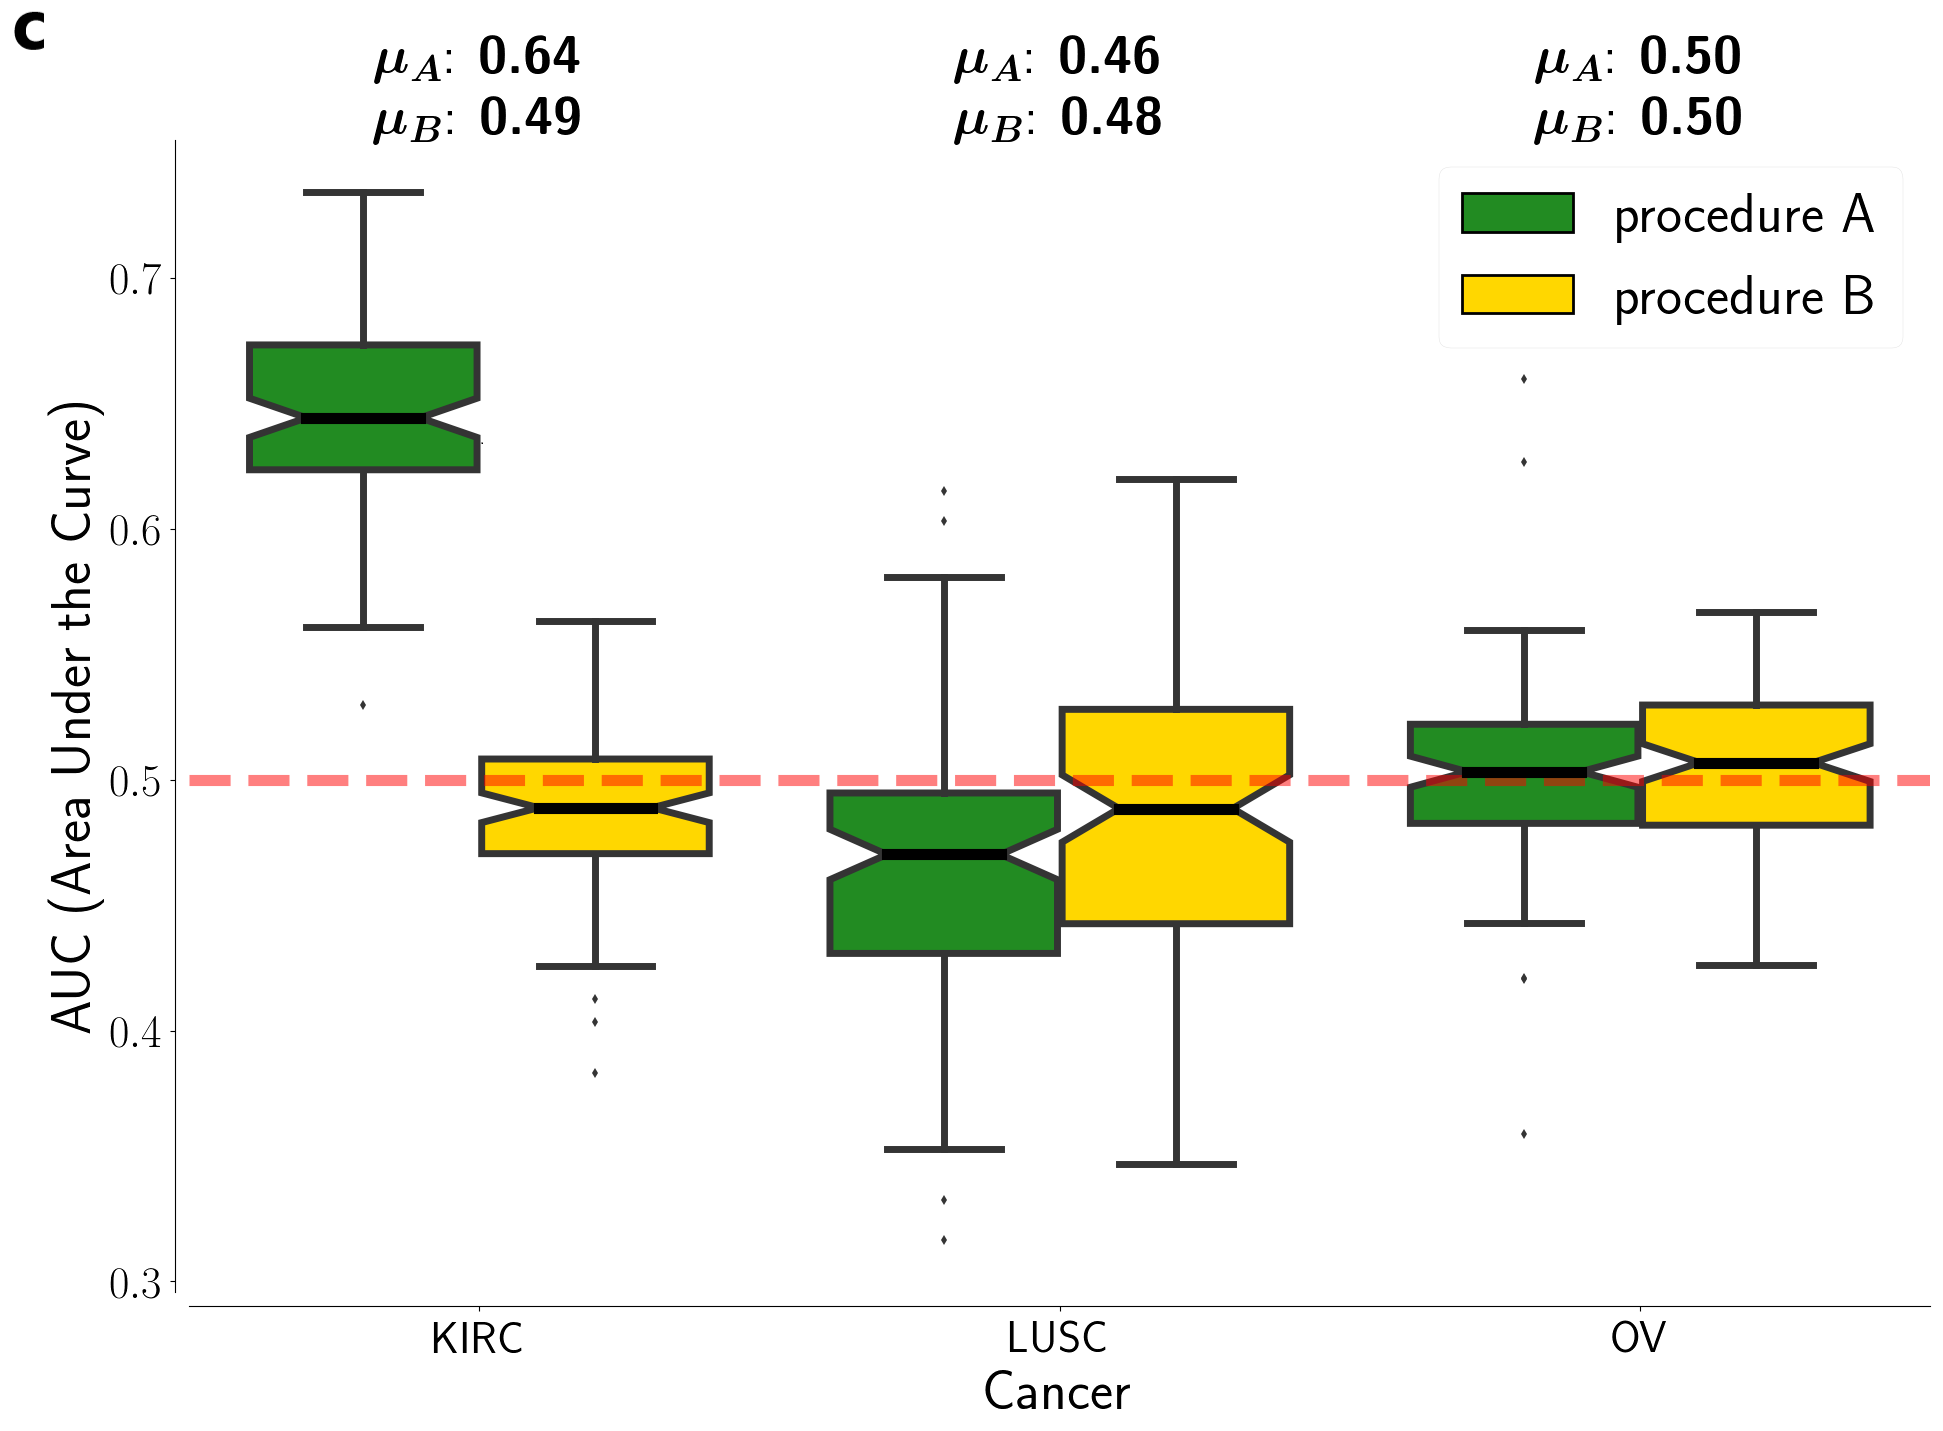
\includegraphics[width=0.4\textwidth]{RPPA_boxplot.png}
\qquad
\centering
\def\svgwidth{0.45\textwidth}
\input{./img/RPPA_tables.pdf_tex}
\caption{Results obtained by the DNetPRO algorithm pipeline on the four Synapse miRNA and RPPA tumors datasets.
\textbf{(a, c)} Distributions of AUC scores obtained over the four datasets.
Green box-plots: results using procedure $A$ of DnetPRO; yellow box-plots: results obtained using procedure $B$.
\textbf{(b, d)} Comparison of DNetPRO with the methods used in~\cite{Yuan2014}.
The reported values are the max AUC values obtained over the 10-Fold cross-validation procedure.
}
\label{fig:other_results}
\end{figure}

The results obtained on the miRNA dataset (Fig.~\ref{fig:other_results} (a, b)) are comparable to the reference, while for the RPPA dataset only the LUSC tumor shows AUC values comparable with the others.
Moving from the procedure $A$ to the procedure $B$, i.e. adding a second cross-validation step, the RPPA performances drastically decrease for the KIRC and OV, while their remain quite stable for the LUSC dataset.
The same behavior is shown in the miRNA datasets in which however both performances are still comparable or better (KIRC, GBM, LUSC) than the reference ones.

These results are not so good as the mRNA ones and this behavior highlights some limitations of the algorithm.
In the mRNA dataset we hypothesized a monotonic behavior of genes (up- or down-regulation of gene expression level) and this model is very likely.
An analogous model for the miRNA data has not yet been demonstrated.
We can guess that the low performances obtained on the RPPA were related to the intrinsic nature of these data and to the experimental difficulties about data interpretation.


\end{document}
